\section{Bernie Stone Case Study}
\begin{frame}{Bernie Stone Case Study | Background}
    \begin{itemize}
        \item Bernie Stone was an alderman in Chicago's 50th ward from 1973-2011. 
        \item He was a member of the infamous ``Vrdolyak 29'' -- a group of aldermen who opposed Mayor Harold Washington in the 1980s.
        \item Two of his campaign employees, Anish Eapen and Armando Ramos were charged with vote fraud in 2008
        \item He was well-known in the community for his ``political philosophy'' and Rahm Emanuel described him as ``fiercely loyal to his constituents''
    \end{itemize}
    \begin{quotation}
        ``You take care of the people who take care of you, you know, the people who voted for you, That's not Chicago politics, that's politics 101''
    \end{quotation}
    \raggedleft{ -Alderman Bernie Stone (50th ward)}
\end{frame}

\begin{frame}{Bernie Stone Case Study | Supporting Precincts}
Below are some of the precincts that supported Bernie Stone in the 2007 election and with campaign contributions over the 2005-2011 period.
\begin{figure}[H]
    \centering
    % First subfigure
    \begin{subfigure}[b]{0.3\textwidth} % Adjusted width
    \includegraphics[width=\textwidth]{input/contribution_map_stone_ward_50_2003_2011.png}
    \caption{Campaign contributions to Alderman Stone, 2003-2011}
    \end{subfigure}
    % Second subfigure
    \begin{subfigure}[b]{0.3\textwidth} % Adjusted width
    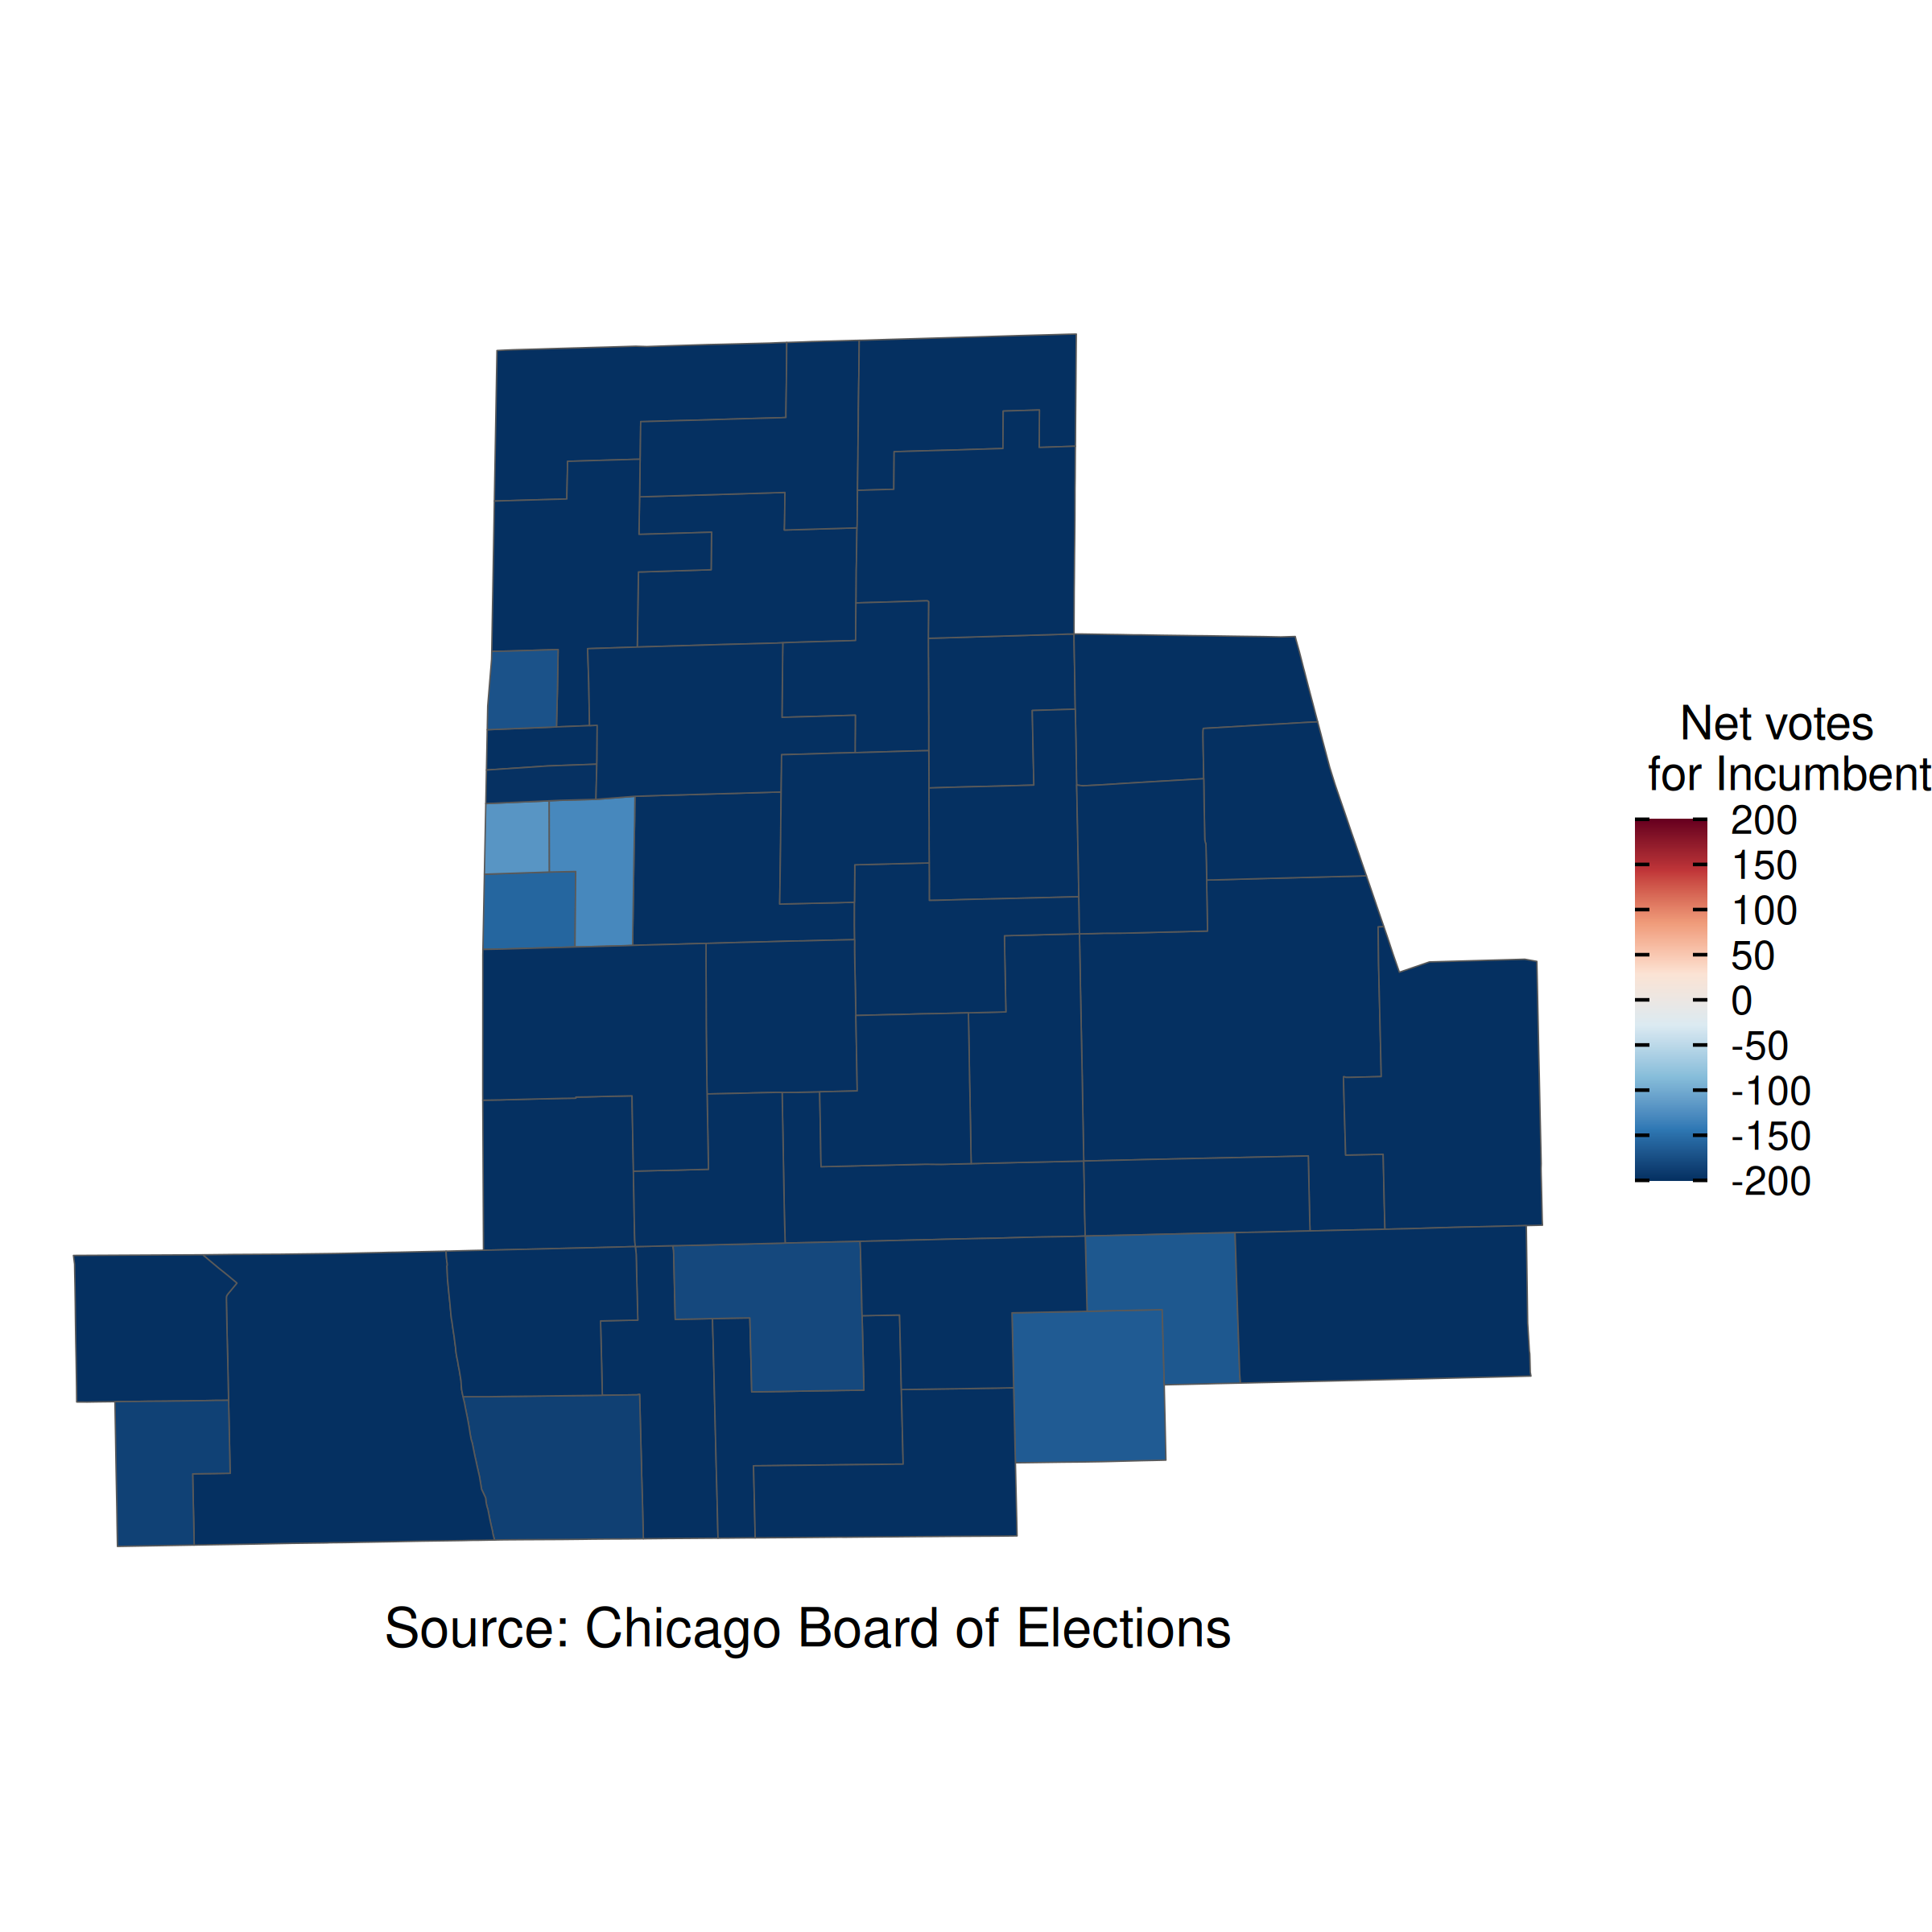
\includegraphics[width=\textwidth]{input/ward_50_2007_runoff_incumbent_precinct_results.png}
    \caption{Net votes for Alderman Stone, 2007}
    \end{subfigure}
    \caption{Distribution of Spending per Precinct for both ward maps in the dataset}
    \label{fig:stone_support_maps}
\end{figure}
\end{frame}

\begin{frame}{Bernie Stone Case Study | Spending Time Series}
Figure\ref*{fig:stone_spending_timeline} shows the average spending per precinct for the top and bottom 8 precincts in the 50th ward by campaign contributions.
This is the first time that this data has been publicly shown.
    \begin{figure}[H]
        \centering
        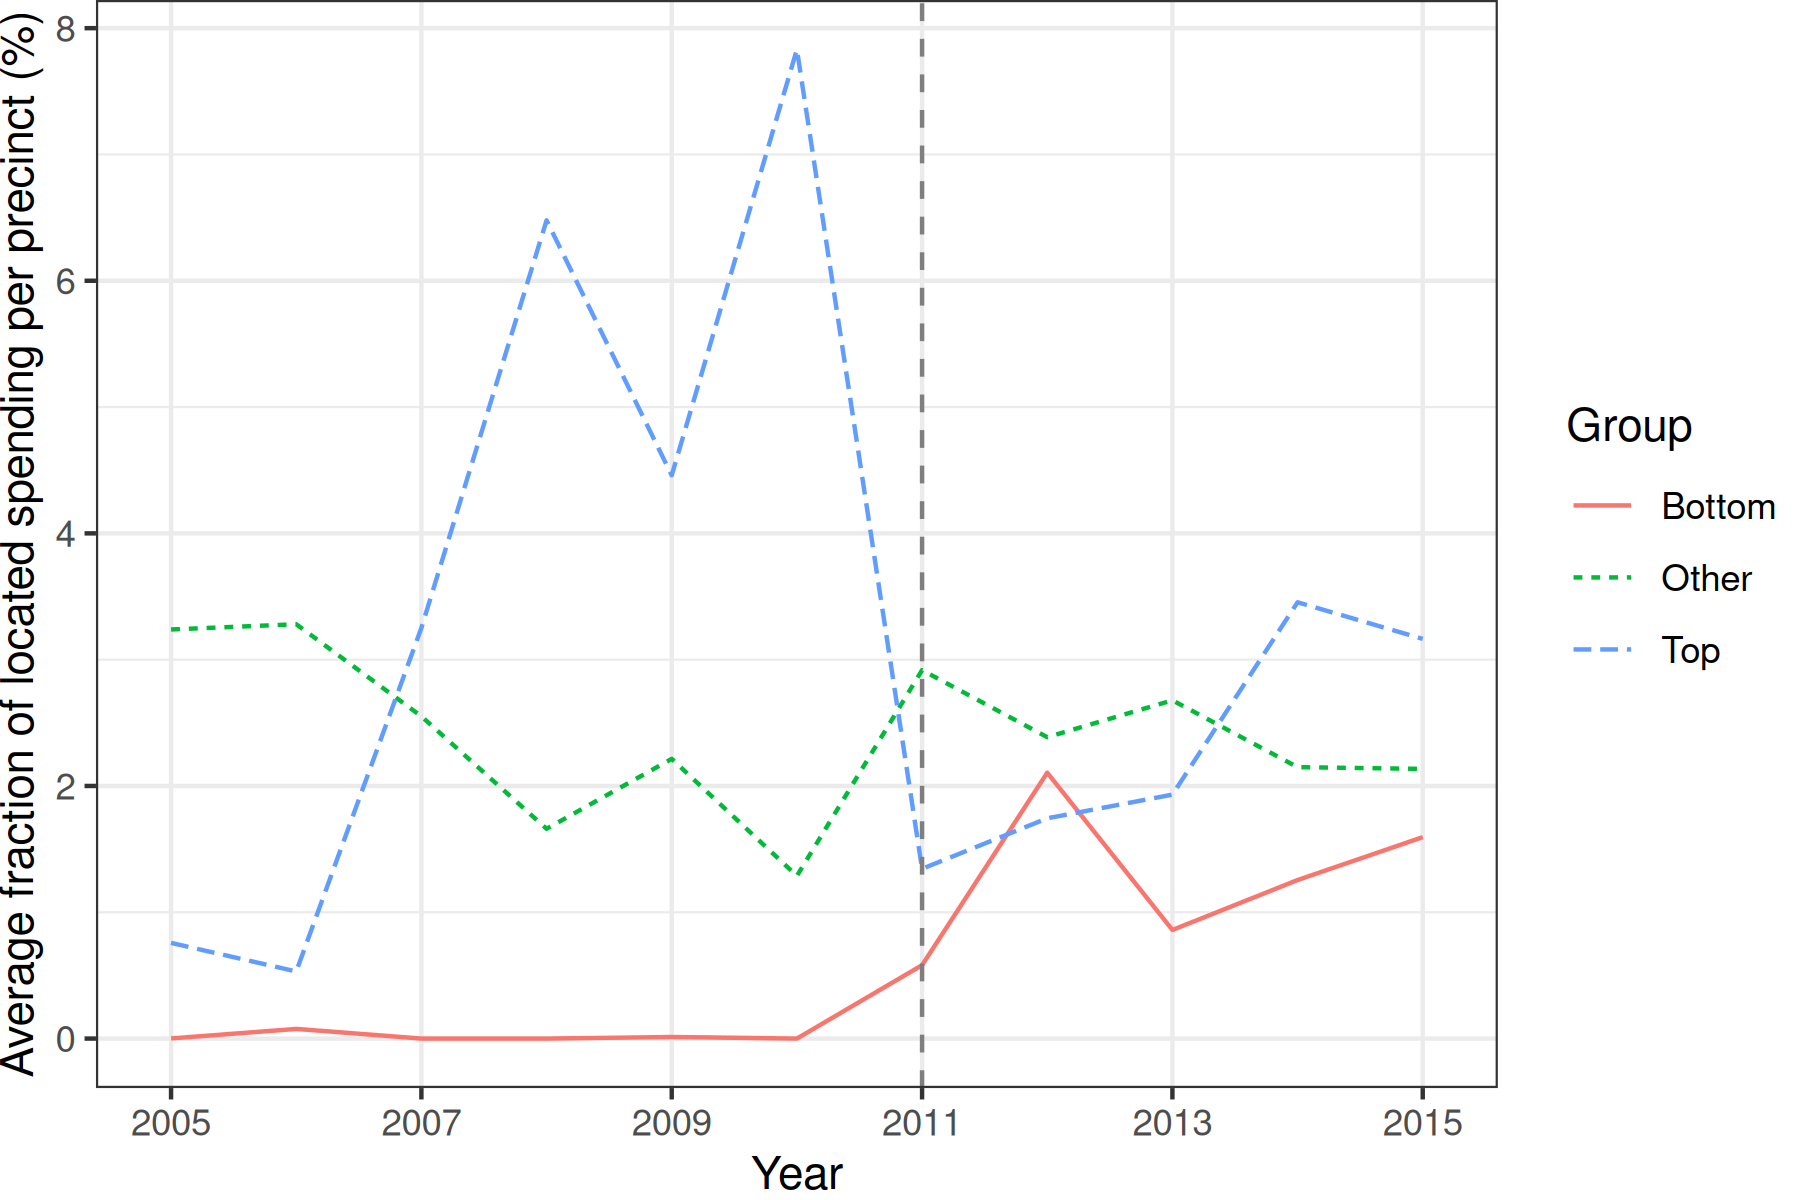
\includegraphics[width=0.4\textwidth]{input/ward_50_contribution_8_precincts_timeline.png}
        \caption{Average Spending per Precinct in the 50th Ward, 2005-2016}
        \label{fig:stone_spending_timeline}
    \end{figure}
\end{frame}

\begin{frame}{Bernie Stone Case Study | Spending Map}
Figure\ref*{fig:stone_menu_maps} compares the chosen distributions of spending before and after Bernie Stone was defeated in 2011.
    \begin{figure}[H]
        \centering
        % First subfigure
        \begin{subfigure}[b]{0.3\textwidth} % [b] aligns at the bottom
        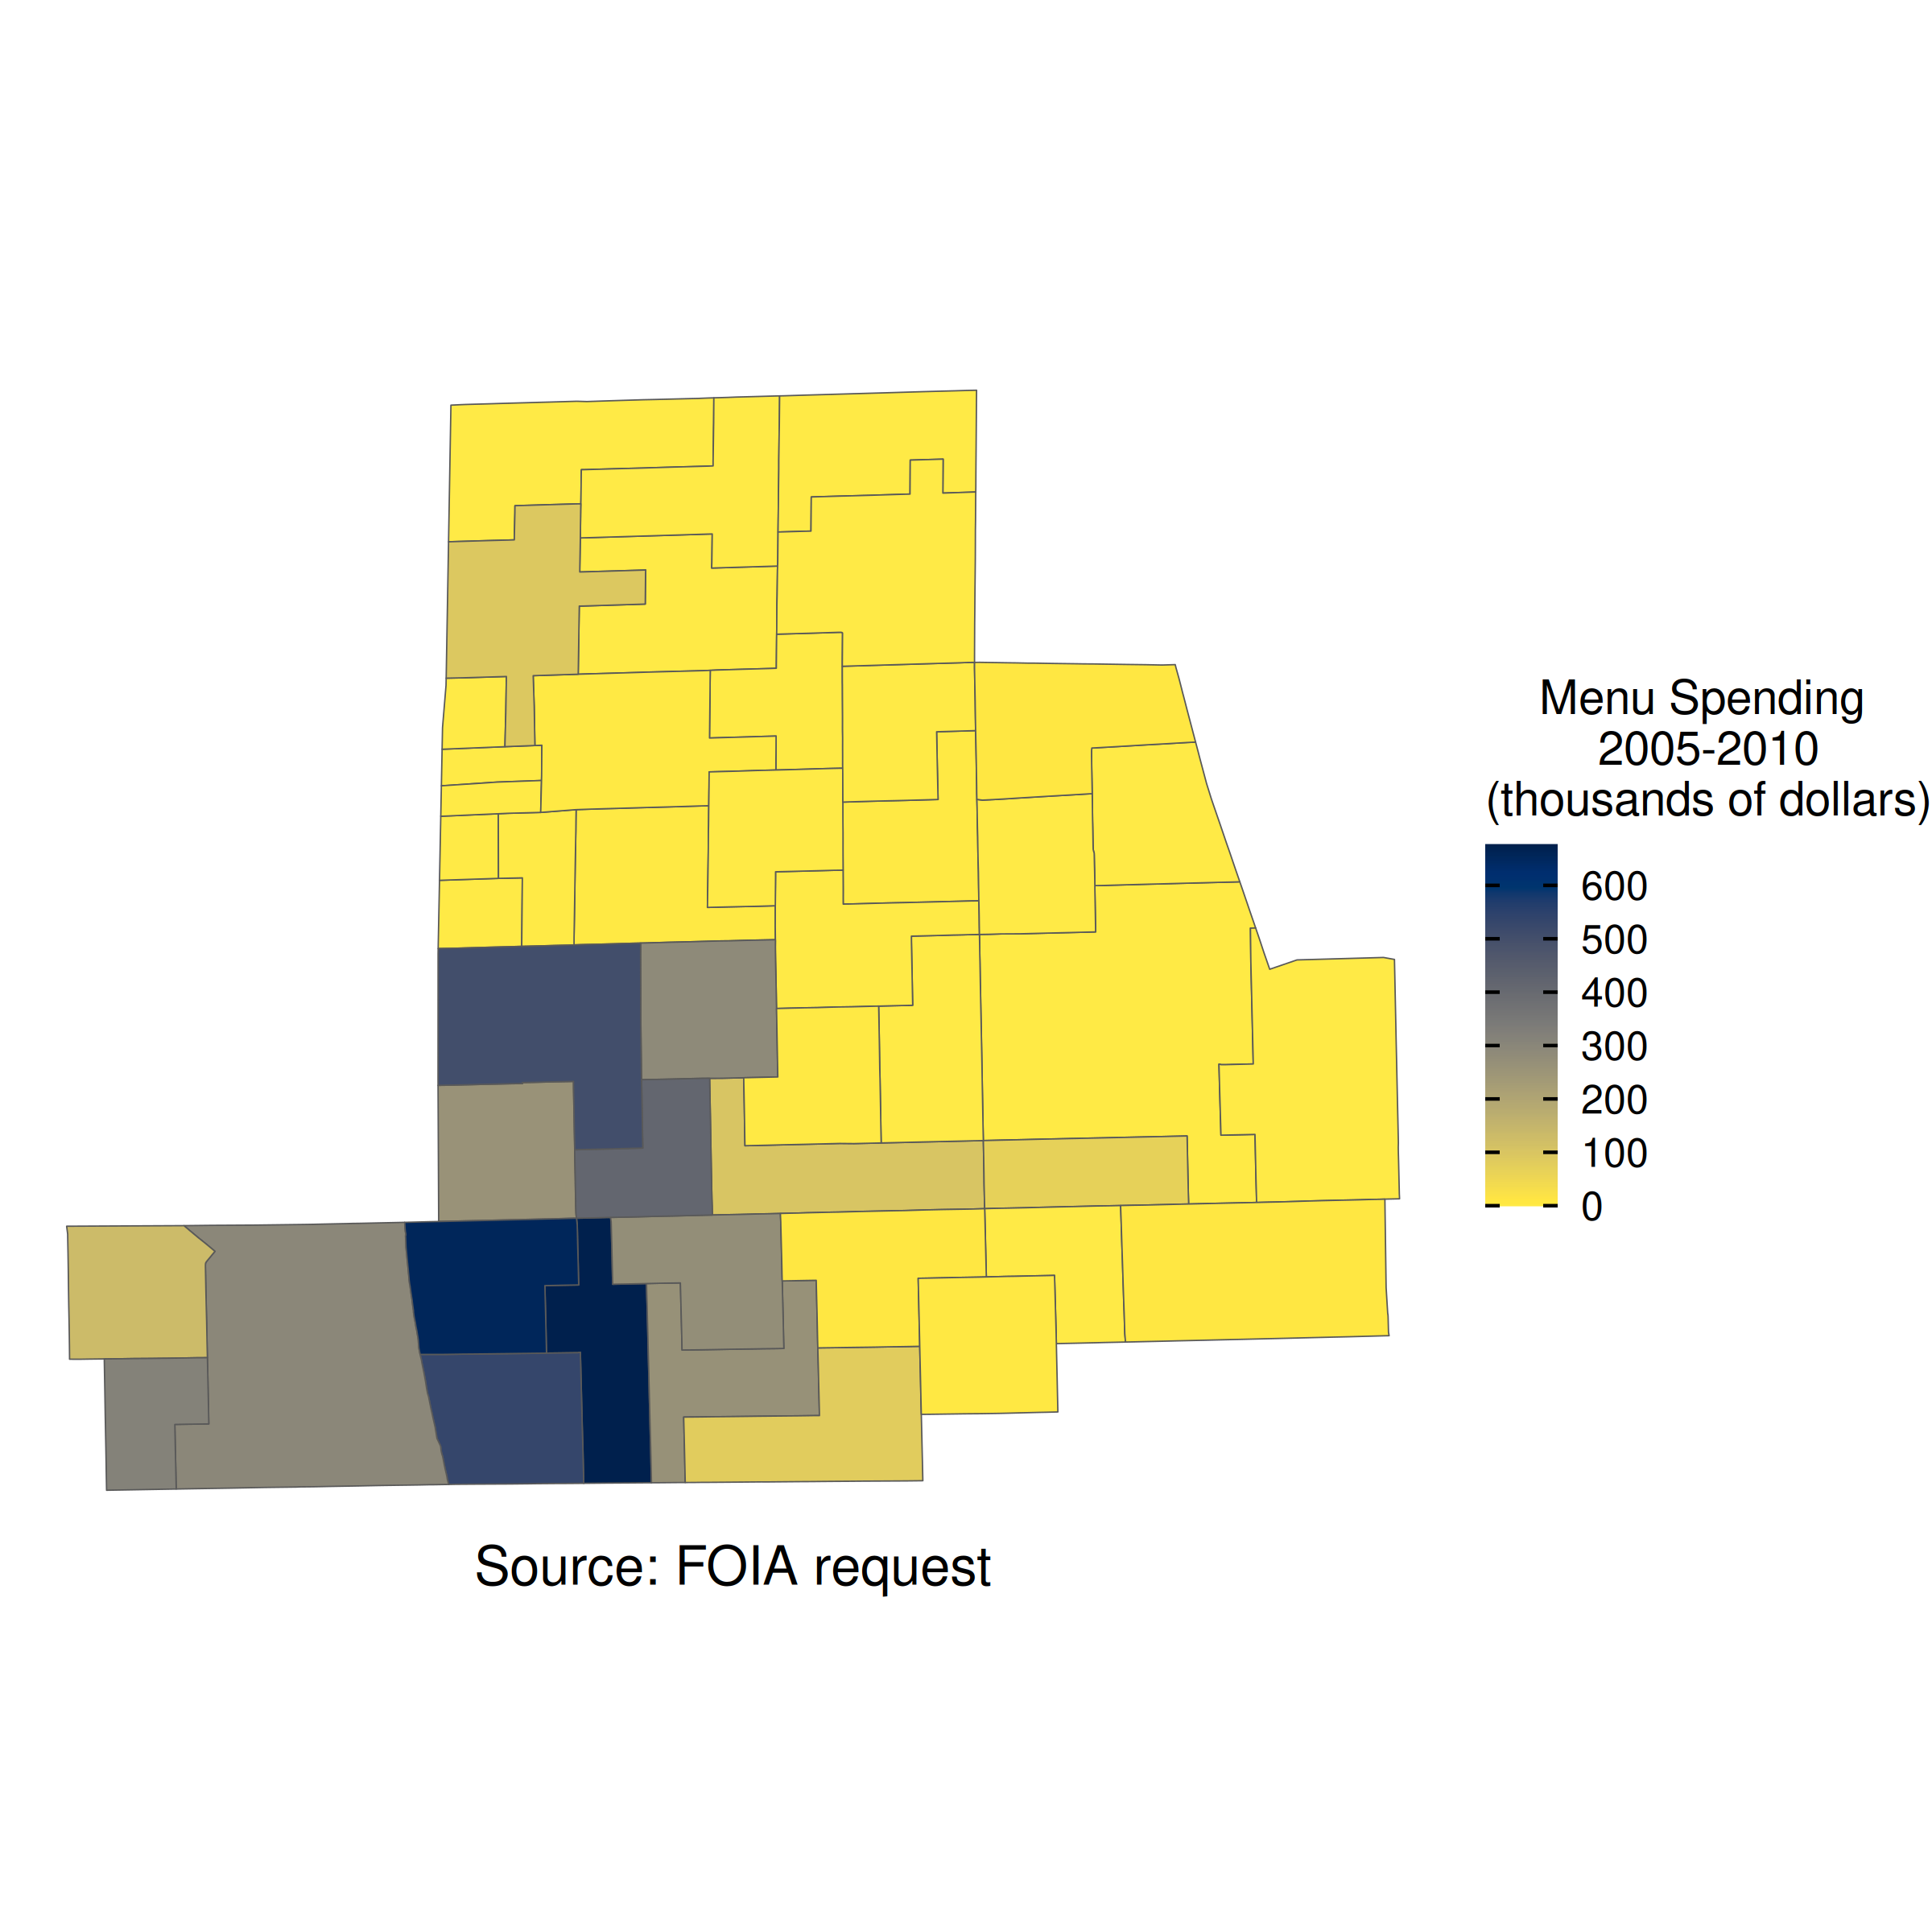
\includegraphics[width=\textwidth]{input/ward_50_menu_map_2005_2010.png}
        \caption{50th Ward Menu Allocation, 2005-2010}
        \end{subfigure}
        % Second subfigure
        \begin{subfigure}[b]{0.3\textwidth}
        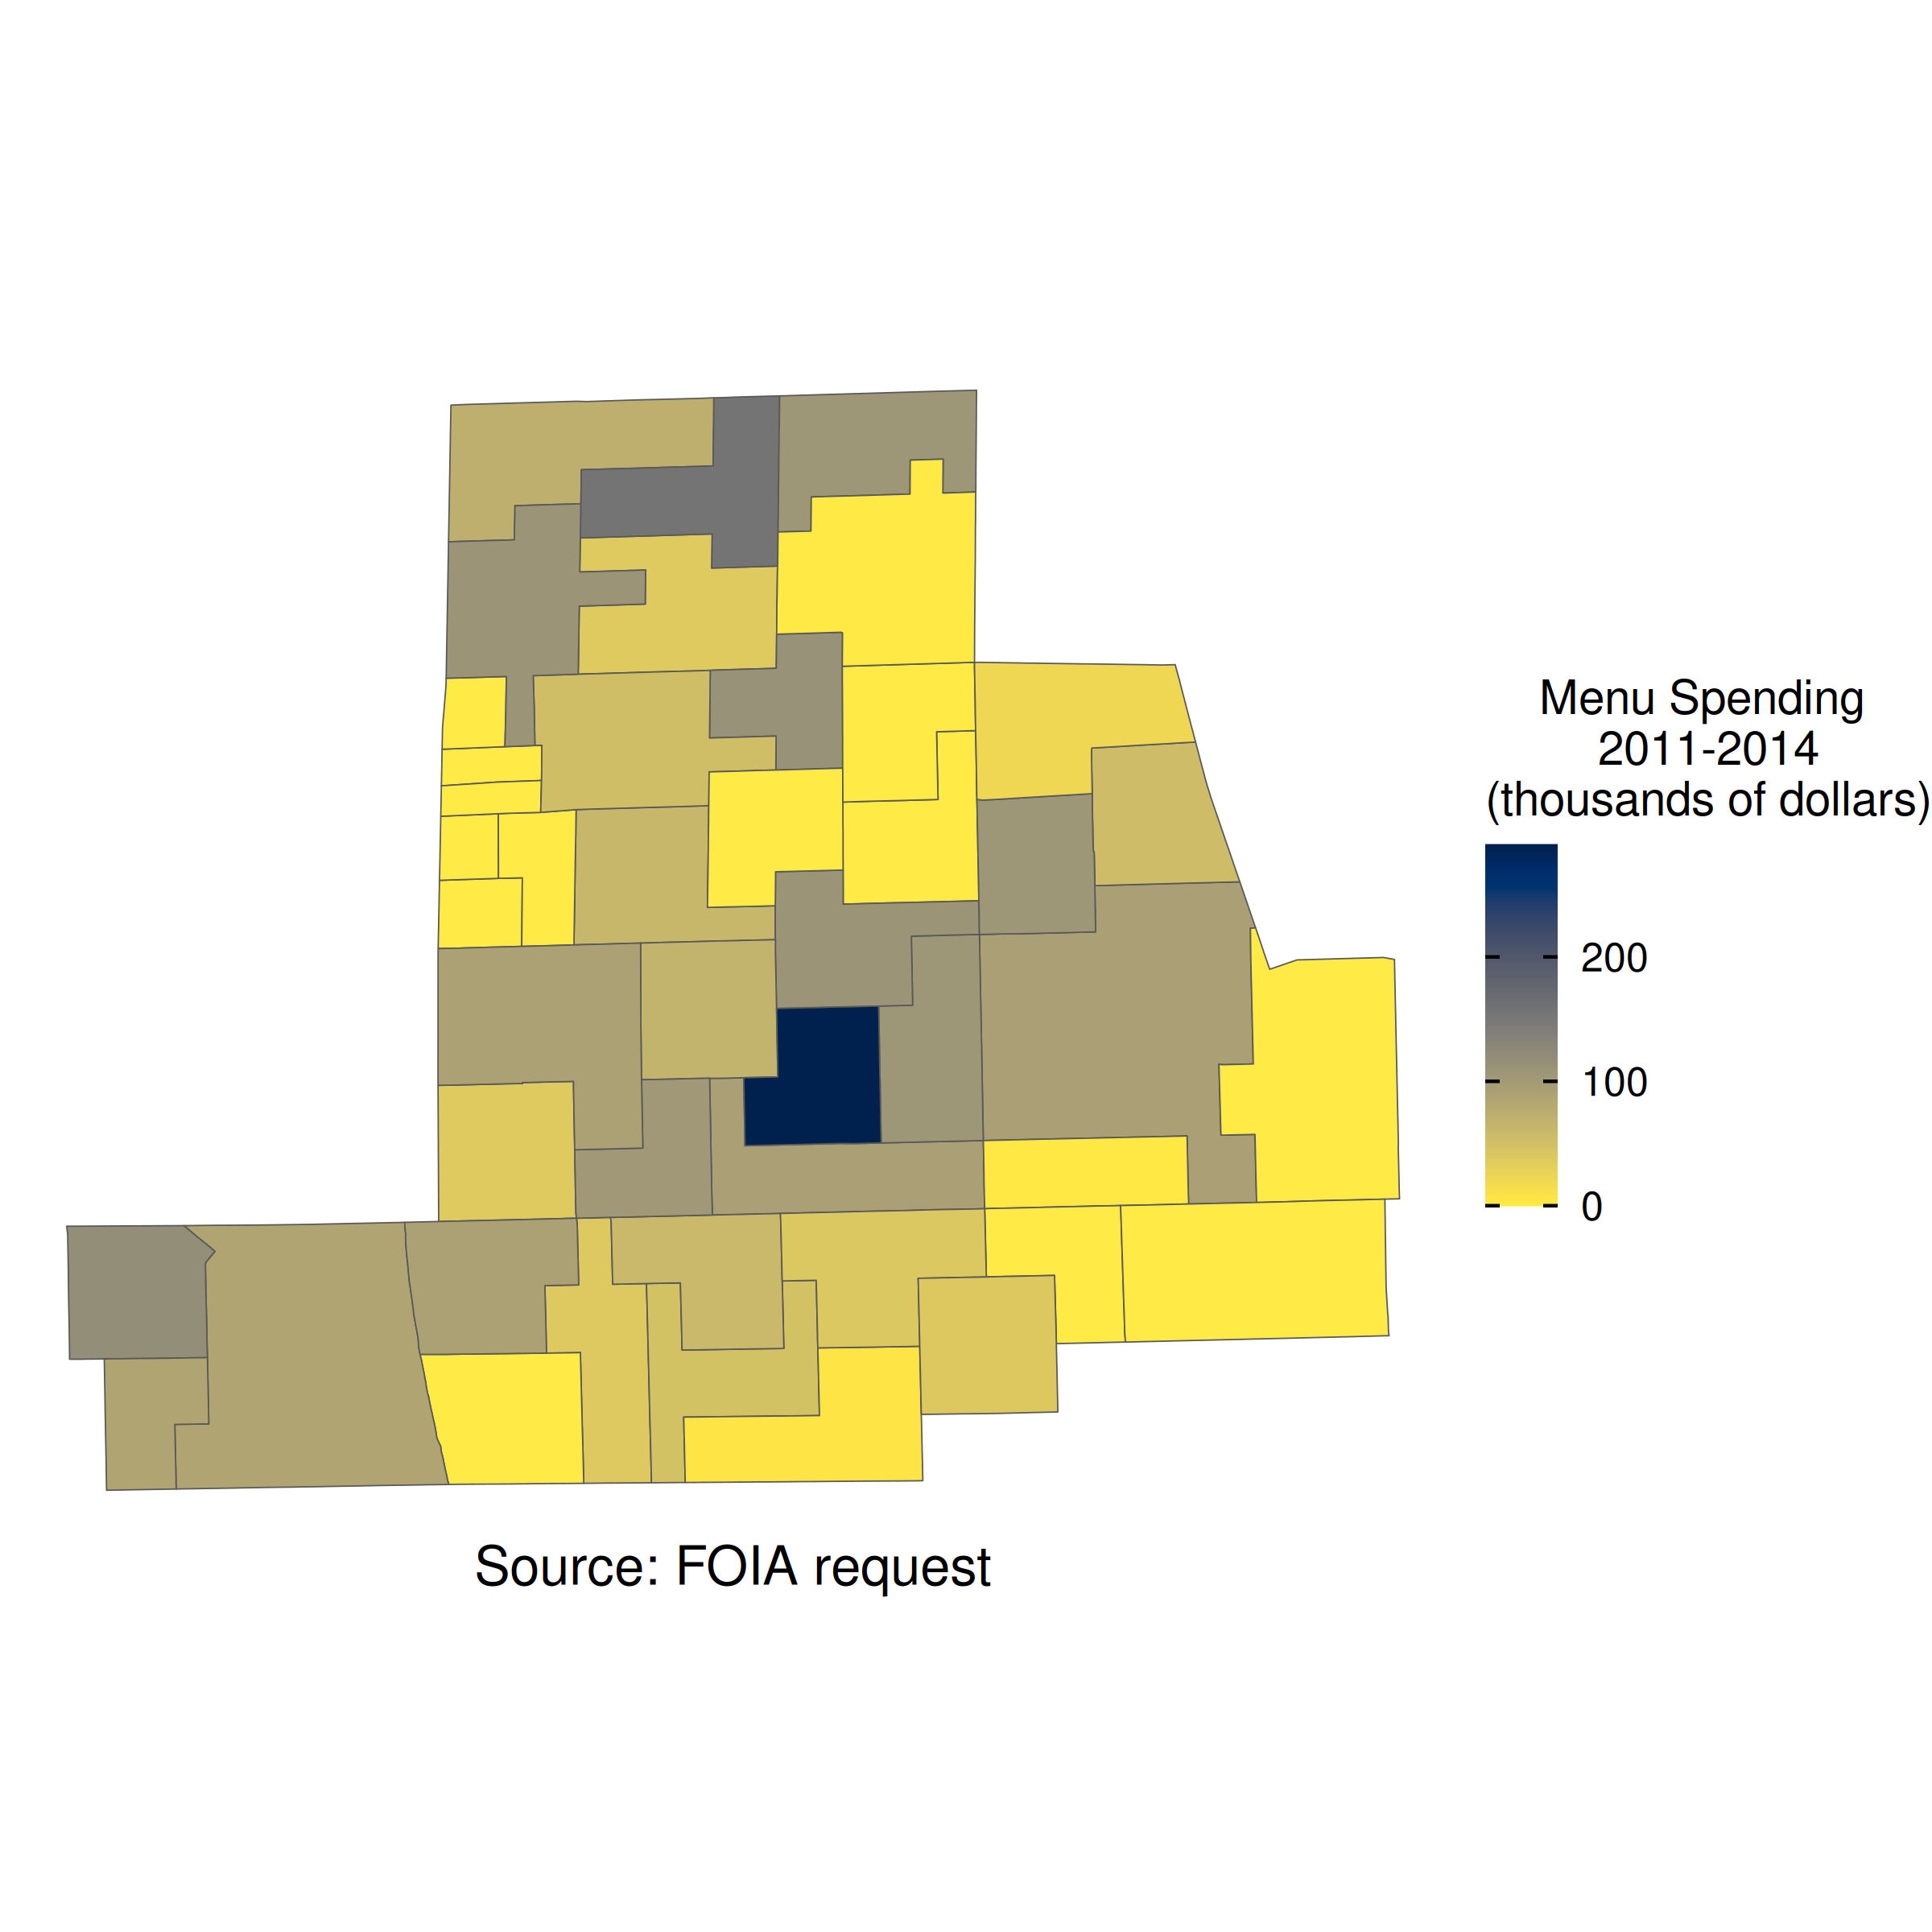
\includegraphics[width=\textwidth]{input/ward_50_menu_map_2011_2014.png}
        \caption{50th Ward Menu Allocation, 2011-2015}
        \end{subfigure}
        \caption{50th Ward Menu Allocation, 2011-2016}
        \label{fig:stone_menu_maps}
    \end{figure}
\end{frame}
